\documentclass[geosciences,article,submit,moreauthors,pdftex]{Definitions/mdpi} 

% If you would like to post an early version of this manuscript as a preprint, you may use preprint as the journal and change 'submit' to 'accept'. The document class line would be, e.g., \documentclass[preprints,article,accept,moreauthors,pdftex]{mdpi}. This is especially recommended for submission to arXiv, where line numbers should be removed before posting. For preprints.org, the editorial staff will make this change immediately prior to posting.

%---------
% article
%---------
% The default type of manuscript is "article", but can be replaced by: 
% abstract, addendum, article, benchmark, book, bookreview, briefreport, casereport, changes, comment, commentary, communication, conceptpaper, conferenceproceedings, correction, conferencereport, expressionofconcern, extendedabstract, meetingreport, creative, datadescriptor, discussion, editorial, essay, erratum, hypothesis, interestingimages, letter, meetingreport, newbookreceived, obituary, opinion, projectreport, reply, retraction, review, perspective, protocol, shortnote, supfile, technicalnote, viewpoint
% supfile = supplementary materials

%----------
% submit
%----------
% The class option "submit" will be changed to "accept" by the Editorial Office when the paper is accepted. This will only make changes to the frontpage (e.g., the logo of the journal will get visible), the headings, and the copyright information. Also, line numbering will be removed. Journal info and pagination for accepted papers will also be assigned by the Editorial Office.

%------------------
% moreauthors
%------------------
% If there is only one author the class option oneauthor should be used. Otherwise use the class option moreauthors.

%---------
% pdftex
%---------
% The option pdftex is for use with pdfLaTeX. If eps figures are used, remove the option pdftex and use LaTeX and dvi2pdf.

%=================================================================
\firstpage{1} 
\makeatletter 
\setcounter{page}{\@firstpage} 
\makeatother
\pubvolume{TBDXX}
\issuenum{TBDYY}
\articlenumber{TBDZZ}
\pubyear{2021}
\copyrightyear{2021}
\externaleditor{Academic Editor: Dr. Rafael Tinoco}
\history{Received: date; Accepted: date; Published: date}
%\updates{yes} % If there is an update available, un-comment this line

%% MDPI internal command: uncomment if new journal that already uses continuous page numbers 
%\continuouspages{yes}

%------------------------------------------------------------------
% The following line should be uncommented if the LaTeX file is uploaded to arXiv.org
%\pdfoutput=1

%=================================================================
% Add packages and commands here. The following packages are loaded in our class file: fontenc, calc, indentfirst, fancyhdr, graphicx, lastpage, ifthen, lineno, float, amsmath, setspace, enumitem, mathpazo, booktabs, titlesec, etoolbox, amsthm, hyphenat, natbib, hyperref, footmisc, geometry, caption, url, mdframed, tabto, soul, multirow, microtype, tikz

\newcommand\Rey{\mathrm{Re}}

\usepackage{siunitx}
\DeclareSIUnit\year{yr}

\usepackage{textcomp}

\usepackage{threeparttable}
\usepackage{longtable}

%=================================================================
%% Please use the following mathematics environments: Theorem, Lemma, Corollary, Proposition, Characterization, Property, Problem, Example, ExamplesandDefinitions, Hypothesis, Remark, Definition, Notation, Assumption
%% For proofs, please use the proof environment (the amsthm package is loaded by the MDPI class).

%=================================================================
% Full title of the paper (Capitalized)
\Title{Sediment Interception by Emergent Stems Across Varying Patch Densities and Flows}

% Author Orchid ID: enter ID or remove command
\newcommand{\orcidauthorA}{0000-0002-7970-841X} % Add \orcidA{} behind the author's name
%\newcommand{\orcidauthorB}{0000-0000-000-000X} % Add \orcidB{} behind the author's name

% Authors, for the paper (add full first names)
\Author{Jordan Wingenroth $^{1}$*\orcidA{}, Candace Yee $^{2}$, Justin Nghiem$^{1,3\dagger}$ and Laurel Larsen $^{1,2}$}

% Authors, for metadata in PDF
\AuthorNames{Jordan Wingenroth, Candace Yee, Justin Nghiem and Laurel Larsen}

% Affiliations / Addresses (Add [1] after \address if there is only one affiliation.)
\address{%
$^{1}$ \quad Department of Geography, University of California, Berkeley, CA

$^{2}$ \quad Department of Civil and Environmental Engineering, University of California, Berkeley, CA

$^{3}$ \quad Department of Statistics, University of California, Berkeley, CA}

% Contact information of the corresponding author
\corres{Correspondence: j.wingenroth@berkeley.edu}

% Current address and/or shared authorship
\firstnote{Current address: California Institute of Technology, Pasadena, CA} 
%\secondnote{These authors contributed equally to this work.}
% The commands \thirdnote{} till \eighthnote{} are available for further notes

%\simplesumm{} % Simple summary

%\conference{} % An extended version of a conference paper

%TODO
% Abstract (Do not insert blank lines, i.e. \\) 
\abstract{Suspended sediment collected by vegetation in marshes and wetlands contributes to vertical accretion, an important factor in these habitats' futures as sea level rise progresses. Effective capture efficiency (ECE) is a key variable in determining the significance of direct interception in elevation-change models, and one that is not yet thoroughly understood in transitionally turbulent flows. Here we used laboratory flume experiments to determine that ECE decreases with increasing collector Reynolds number (study range: 66 to 200; p < 0.05 for 2 of 3 treatments) and collector density (solid volume fraction: 0.22\% to 1.17\%; p < 0.05 for 2 of 3 treatments), and that biofilm has a considerable positive effect on ECE. This is in agreement with previous similar studies. By combining our data with those of the most similar study, we also present a preliminary model quantitatively assessing the effect of collector density on ECE.}

% Keywords
\keyword{sediment transport; collector efficiency; submerged vegetation; transitional turbulence; biofilm; sedimentation}


\begin{document}

\section{Introduction}

\subsection{Environmental Significance}

Sediment transport is a driver of many key processes in coastal ecosystems, impacting land progradation \cite{kenyon1985morphology}, water quality \cite{goodwin2003temporal}, and ecological productivity \cite{kirwan2007coupled}. With the prospect of climate change and sea level
rise looming, the significance of sediment load to coastal lands has grown considerably. Britsch
and Dunbar \cite{britsch1993land} found that an estimated 17.8\% of land throughout a study area in the Louisiana Coastal
Plain was lost from the 1930s to 1990, with a maximum rate of land loss of about \SI{109}{\kilo\metre\squared/\year}. This trend will be compounded in the near future as rates of relative sea level
rise increase \cite{fitzgerald2008coastal}. Coastal and
deltaic zones are home to a large human population worldwide, on the order of hundreds of millions, and represent a rich social and economic network \cite{syvitski2009sinking}. Developing better understanding of the interplay between geomorphology, ecology, and society in low-elevation deltas, marshes, and wetlands \cite{langley2009elevated, silliman2012degradation, ma2018ecogeomorphic} is an important motivator for future research dedicated to climate change adaptation and mitigation. Sedimentation drivers are an especially important study topic because of their potential for use in management seeking to counteract sea level rise.

Mechanisms by which plants are known to affect sedimentation include direct capture of sediment on stems, leaves, and other plant surfaces \cite{mudd2010does}, direct deposition of organic matter via root growth and shedding of plant matter (e.g., leaves, seeds, fruit) \cite{nyman2006marsh, neubauer2008contributions}, and effects on turbulence and flow patterns impacting the rate at which suspended particles settle out of the water column due to gravity \cite{christiansen2000flow, leonard1995flow}. Additionally, plants' effects on bedload transport have been the subject of numerous studies \cite[e.g.,][]{yager2013influence, yang2019impact, jordanova2003experimental}. These mechanisms act on different, but sometimes overlapping, portions of a water body's sediment load. For instance, settled particles subsequently become bedload, subject to those vegetative effects. Bedload can also be resuspended by turbulent flow, and vegetation has been found to strongly influence the mechanisms by which this occurs also \cite{tinoco2018turbulence}. Even among suspended particles alone, different mechanisms affect particles with different sizes, specific gravity, and surficial properties. While gravitational settling plays a dominant role for large or dense particles in typical flow conditions for vegetated reaches \cite{mudd2010does, leonard1995flow}, fine particles that travel over great longitudinal distances before settling may be destined to either impact vegetation and be collected directly, or pass through vegetated areas without being retained.

\subsection{Theoretical Background}

Capture efficiency ($\eta=\frac{b}{d_c}$) is defined as the ratio between the upstream width ($b$) of the streamlines that encounter a collector and the collector's own diameter ($d_c$) (Figure \ref{fig:capeff}). It is a geometrical parameter that describes the ability of a vegetation stem to collect sediment particles from upstream in a given flow field. Effective capture efficiency ($\eta^\prime=p_r\eta$; ECE) accounts for the fact that not all particles coming into contact with a collector will adhere to it, thus including probability of retention ($p_r$) as a multiplicand in its calculation. ECE is the appropriate variable for the empirical estimates made by our study and presumably any others that involve $p_r$ as an implicit factor, and it, rather than $\eta$, corresponds to the realized efficiency of natural vegetation for removing sediment from flow through direct interception.

% Capture diagram figure
\begin{figure}[H]
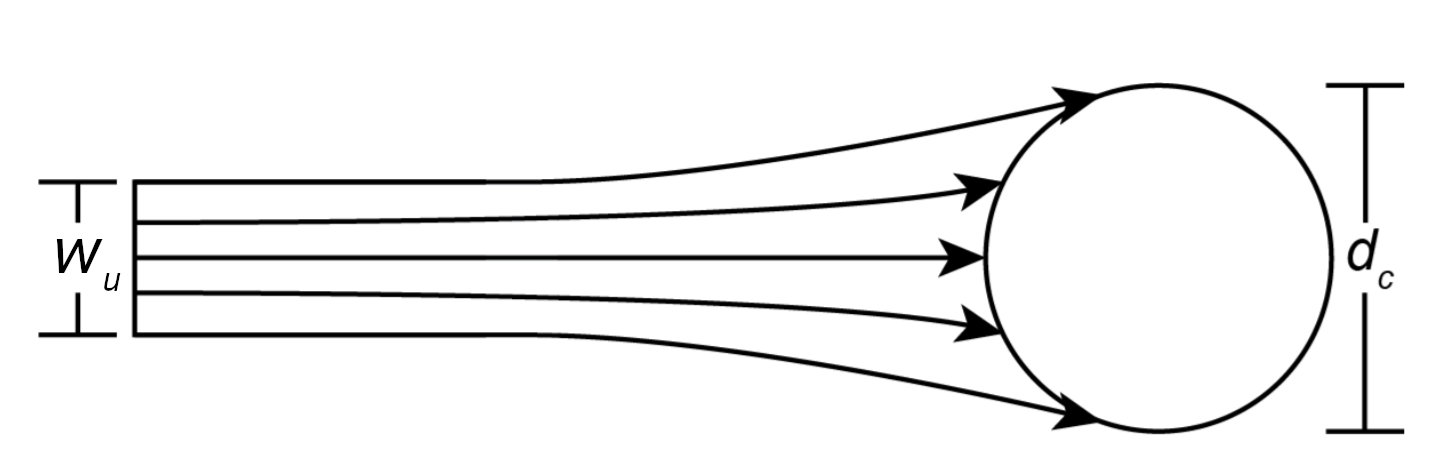
\includegraphics[width=5in]{../pics/collectorefficiency.png}
\centering
\caption{A diagram illustrating capture efficiency for a cylindrical collector. $b$ is the horizontal width of upstream flow and $d_c$ is collector diameter. Adapted from Palmer et al. (2004) \cite{Palmer_2004}.}
\label{fig:capeff}
\end{figure}

Particle capture in transitionally turbulent flows ($1<\Rey<1000$), which occur commonly in the environments and on the length scales of aquatic macrovegetation, does not follow the analytical expressions involving Reynolds number, collector diameter, and particle diameter ($d_p$), derived for creeping flow (REF paper that describes creeping flow solution). For transitional flows (as considered here) and turbulent flows, analytical solutions are intractable so empirical estimates are often employed. Palmer \cite{Palmer_2004} introduced a power law expression for estimating capture efficiency of cylindrical collectors, which takes the form 

\begin{equation}
    \eta=C{\Rey_c}^{a}R^{b}\,,
    \label{eq:powerlaw}
\end{equation}

\noindent where collector Reynolds number $\Rey_c=\frac{ud_c}{\nu}$, $u$ is flow velocity, $\nu$ is kinematic velocity, and $R=\frac{d_c}{d_p}$ is the ratio between collector diameter and particle diameter ($d_p$). $C$, $a$, and $b$ are empirically determined regression coefficients. It is worth noting that Palmer \cite{Palmer_2004} used $\eta$ in their notation for this model as opposed to $\eta^\prime$ because their experiment involved an isolated single cylinder coated with grease, for which retention was assumed to be complete ($p_r = 1$).

Turbulence is also theorized and empirically confirmed to affect the settling velocity of heavy, fine particles \citep{Nielsen_1993, Jacobs_2016, Wang_2018}. Particularly, turbulent eddies generated along a rough bed or within vegetation stands oppose gravitational settling of sediment particles. In addition, turbulent wakes behind individual vegetation stems can remove sediment that has already adhered to neighboring stems (REF paper that described this effect). Thus, sediment-vegetation interaction in transitional flow is two-fold: first, vegetation stems directly intercept sediment from the flow, and second, vegetation structure influences turbulence and thereby gravitational settling.

\section{Materials and Methods}

\subsection{Experimental Methods}

\subsubsection{Materials}

We conducted our experiments in the Ecogeomorphology flume, an indoor (22.2 +/- 1 \SI{}{\celsius}) recirculating flume located in McCone Hall at the University of California, Berkeley. The flume has a rectangular open-channel section (5.25 m L $\times$ 0.6 m W $\times$ 0.6 m H) and a bed and sidewalls that are smooth and transparent (Figure \ref{fig:floorplan}). At its upstream and downstream ends, this section connects to rectangular ducts with gradually changing hydraulic diameter and rounded corners with curved vertical manifolds along streamlines. These features are intended to maintain laminar flow when water is not affected by collectors. Additionally, at the upstream end of the open-channel, a honeycomb flow collimator served to further straighten flow streamlines before water enters the open channel. 



% Flume diagram figure
\begin{figure}[H]
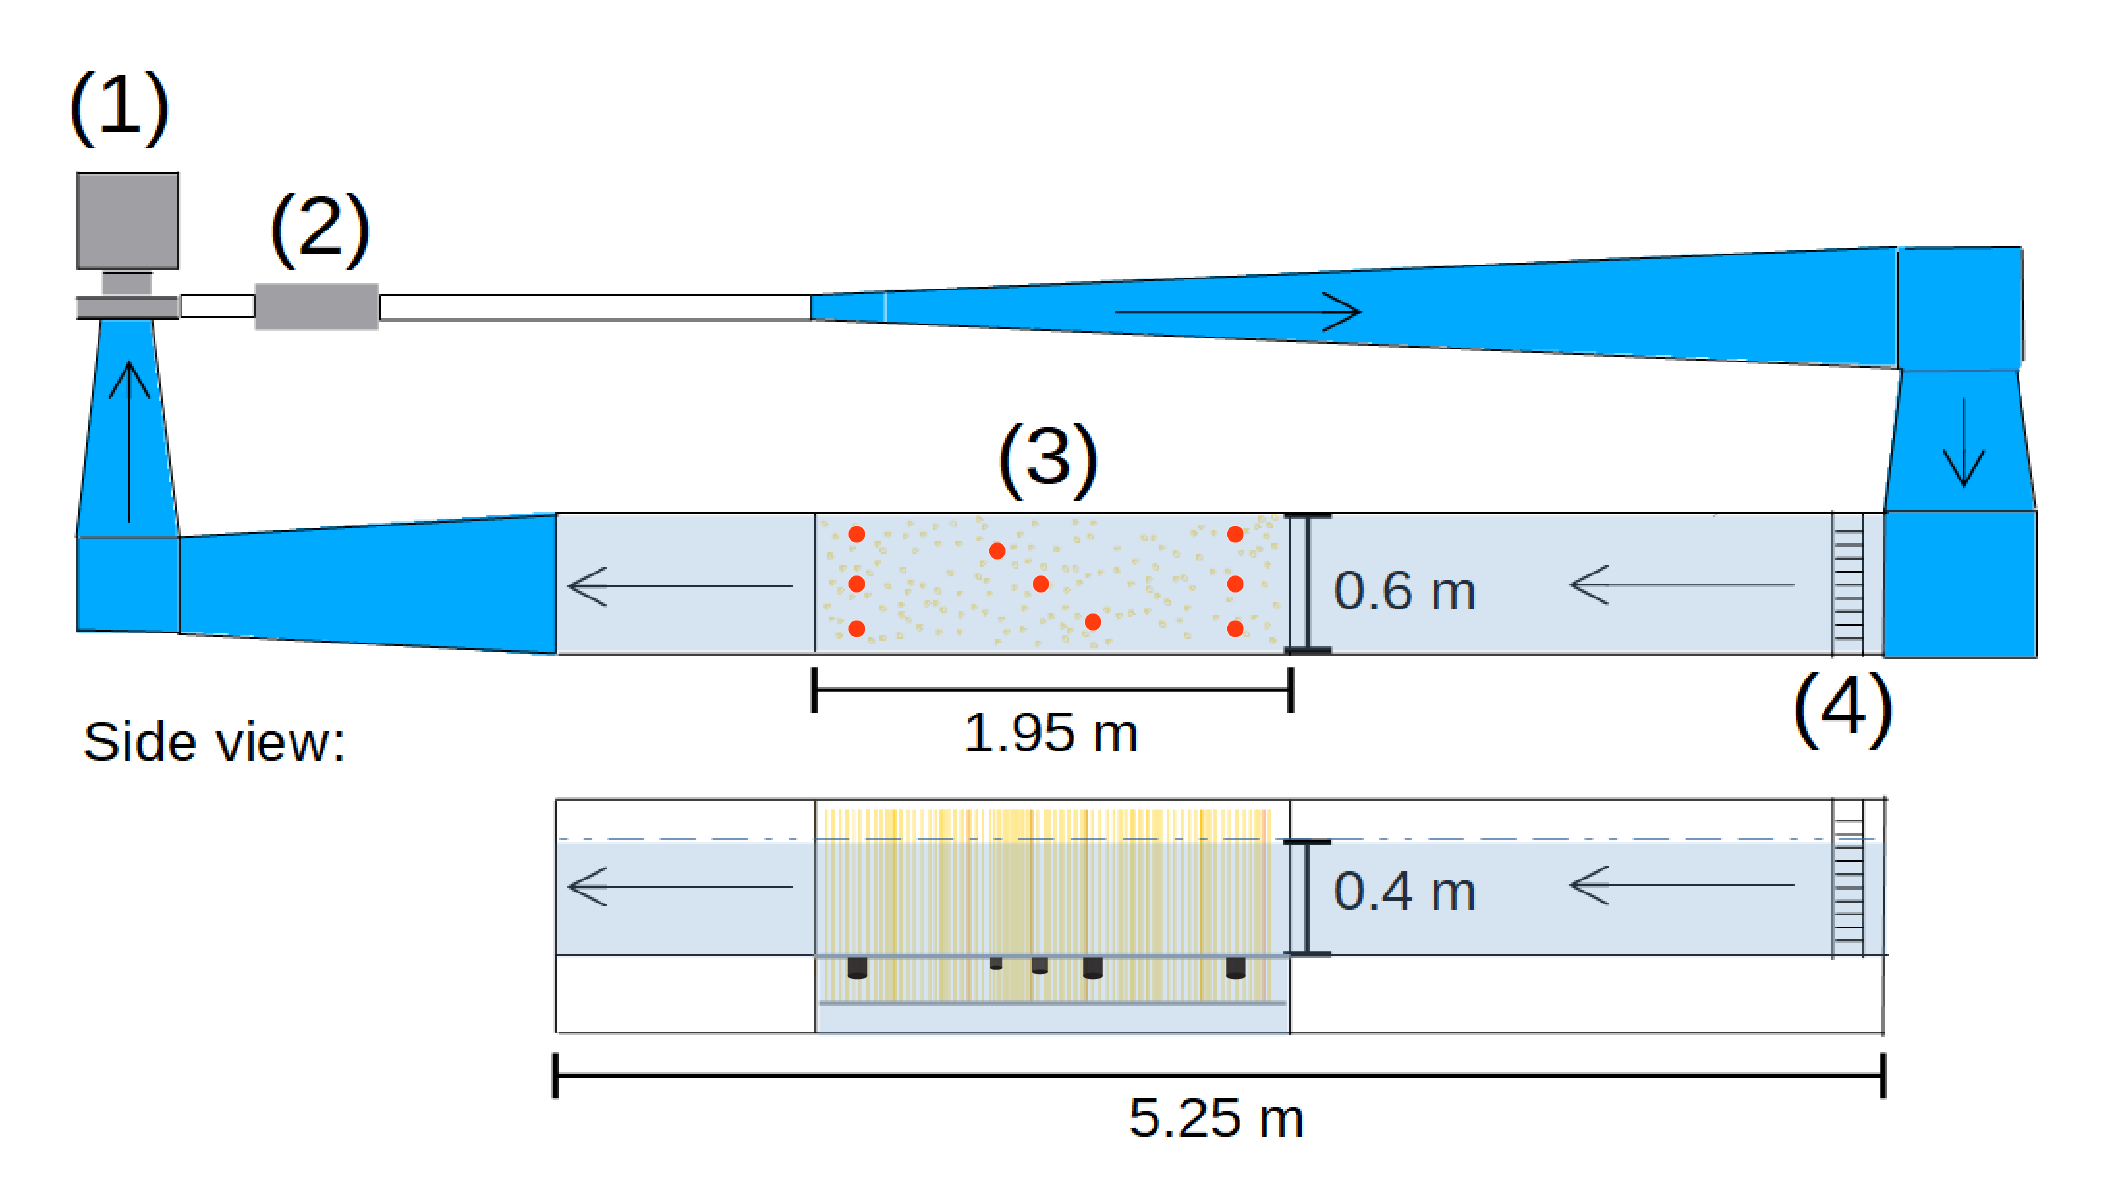
\includegraphics[width=5in]{../pics/flume_with_sedtraps.png}
\centering
\caption{The Ecogeomorphology flume. Not all measurements are to scale. \textbf{(a)} Photograph of the test section (center-left) and pump (right). \textbf{(b)} Conceptual diagram of the flume as seen from above. Labeled parts are: 1) pump, 2) magnetic flowmeter, 3) test section, and 4) honeycomb flow collimator. Arrows indicate direction of flow. Green points represent the inlets for the peristaltic pumps sampling suspended particle concentration. Red areas represent the settling traps. \textbf{(c)} A side view of the open-channel part of the system.}
\label{fig:floorplan}
\end{figure}

In turn, the ducts guide water to and from the inlet and outlet of the pump array, which consists of a disc pump (Discflo Pumps Corporation, Santee, CA), and a magnetic flowmeter, connected by PVC pipe. This type of pump uses rotating discs to generate viscous drag, which entrains fluid and suspended particles through its interior chamber while maintaining laminar flow and avoiding structural disruption, pulsation, and abrasion \cite{discflo}. Altogether, the flume design maintains constant, adjustable discharge through the open channel, minimizing background turbulence and other artifacts that arise with other types of pumps.

Within the open channel, we designated a "test section" 1.95 m in length where collectors would be installed. This test section and the surrounding area were instrumented with the following devices:
\begin{enumerate}
     \item A flat-bedded array positioned flush with the neighboring channel bed, containing vertical, emergent collector stems, which were spaced uniformly in an unpatterned manner
    \item Two battery-operated peristaltic pumps (Cole-Parmer, Vernon Hills, IL) used to sample suspended particle concentration via three hose inlets each (inside diameter = 3.1 mm), which were suspended at a range of heights from the channel bed (5; 14; 27 cm); these were positioned 50 cm upstream and downstream of the test section 
   \item Settling traps (n = 9) with 2.5 cm circular openings flush with the bed and collection filters (Whatman GF/F) on perforated filter holders recessed 5 cm below, which were used to estimate settled particle mass; these were interspersed among the collectors in a grid-like pattern
\end{enumerate}

We used 1/8" (0.3175 cm) cylindrical wooden dowels as collectors, which were covered in silicone grease (Chemplex 710, Fuchs Petrolub, Mannheim, Germany) in order to retain impacted particles. Crushed walnut shell was used as a substitute for suspended sediment because it has surficial and physical properties comparable to the organic-rich types common in wetlands \cite{muller2017experiments, jenzer2015sediment, redding2006particle}. We used WF5-200 grade (Composition Materials Co., Milford, CT), which passes entirely through a \#60 sieve (\SI{250}{\micro\metre}), and which we determined has a average particle diameter ($d_{50}$) of \SI{25.2}{\micro\metre} based on measurements using a laser-scattering-based instrument (LISST-Portable|XR, Sequoia Scientific, Bellevue, WA). We also empirically estimated the particle density for this specific walnut shell flour to be 1.53 \SI{}{\gram/\centi\metre\cubed}.

\subsubsection{Suspended Particle Concentration Analysis}

We conducted experimental runs for a fully-crossed parameter space of collector Reynolds number (67; 134; 200) and collector density (0; 278; 800; 1450 collectors/m$^2$). These values, as well as other experimental parameters held constant throughout, were chosen because they correspond to those that might occur for emergent grasses or reeds in natural settings (Table \ref{tbl:parameters}). A zero-collector control density was included in order to isolate the effects of our experimental installations from the background effects of the rest of the flume.   

% Experimental parameters table
\begin{table}[H]
\caption{Experimental and natural parameter ranges. Natural values are based on approximations or measurements from cited studies and literature reviews in wetlands or other low-elevation flows.}
\centering
\begin{threeparttable}
\begin{tabular}{lcccc}
\toprule
\textbf{Parameter}&\textbf{This study}&\textbf{Fauria et al. (2015)}&\textbf{Purich (2006)}&\textbf{Natural}\\
\midrule
Flow velocity (\SI{}{\centi\metre/\second})     
& 2.0--6.0    & 1.8--6.1    & 1.0--10.2    & 0--25 \cite{nikora2008hydraulic}    \\
Flow depth (\SI{}{\centi\metre})                
& 40          & 14--17      & 12           & 0--50 \cite{kadlec1990}    \\
\midrule
Collector shape
& Cylindrical & Artificial grass  & Cylindrical & Varies \\ 
Collector diameter (\SI{}{\centi\metre})
& 0.318       & 0.3         & 0.6          & 0.1--1.2 \cite{Nepf_2012,wright2018hydrological} \\
Collector Reynolds number                       
& 66--200     & 54--183     & 70--640      & 5--1000 \cite{kadlec1990}  \\ 
Collector density ($\#/\text{m}^2$)
& 278--1450   & 2724--7209  & 1013--4053   & 10--2700 \cite{wright2018hydrological} \\
Solid volume fraction (\%)
& 0.22--1.17  & 0.82--2.16  & 2.86--11.5   & 0.1--1 \cite{Nepf_2012}   \\ 
\midrule
Particle type
& Walnut shell  & Road dust  & Pliolite\textsuperscript{\textregistered}   & Sediment \\ 
Particle density  (\SI{}{\gram/\centi\metre\cubed})    
& 1.53        &2.27--2.61 \tnote{1}  & 1.03         & 1.43--2.39 \cite{redding2006particle} \\
Average particle diameter, $d_{50}$ (\SI{}{\micro\metre})     
& 25.2        & $\sim$10--15 \tnote{2} & 212--250     & 45--100 \cite{hejduk2010variations,noe2010glades}  \\
Suspended concentration (\SI{}{\micro\liter/\liter})      
& 5--55   & 9--50       & $\sim$110   & 2-25 \cite{noe2010glades,aiona2013can}      \\
\midrule
Particle-collector diameter ratio, $R$      
&0.0079       &0.0004--0.083 \tnote{2} & 0.037        & <0.25     \\
\bottomrule
\vspace{-4mm}
\end{tabular}
\begin{tablenotes}
\footnotesize \item[1] Estimated from a different study about road dust properties \cite{mckenzie2008size} 
\vspace{2mm}
\footnotesize \item[2] Fauria et al. \cite{Fauria_2015} used a LISST to measure collection across a broad range of particle diameters (1.25--250 \SI{}{\micro\metre})
\end{tablenotes}
\end{threeparttable}
\label{tbl:parameters}
\end{table}

Before each experiment, the flume was filled with tap water to 0.4 m depth in the test section, which was enough to fully submerge the pump and almost the entirety of the duct length. At this depth, the volume of water in the entire flume was approximately 2.43 m$^3$ (See Supplementary Information).  A Nortek Vectrino Profiler ADV (acoustic Doppler velocimeter; Nortek AS, Vangkroken 2, 1351 Rud, Norway) was used to calibrate the pump to generate channel mean flow velocities (2.0; 4.0; 6.0 \SI{}{\centi\metre/\second}) within the pump's capabilities and corresponding to the range of interest for $\Rey_c$. At these flow rates (0.0048; 0.0096; 0.0144 \SI{}{\metre\cubed/\second}), circulation times for the entire system were 506 s, 253 s, and 169 s, respectively. The drag caused by collectors was not found to detectably affect upstream or downstream flow velocities.

Settling traps were installed immediately before each run, then a slurry consisting of 200 g of crushed walnut shell suspended in 15.1 L of tap water was added using a spigot calibrated to finish draining after a period roughly equal to circulation time (3 minutes). Channel velocity was kept at 6 cm/s for this period across $\Rey_c$ treatments, then adjusted to the appropriate value for the treatment. This procedure was intended to make particle concentration longitudinally even throughout the system. Estimated depth-averaged starting concentration was 82.3 mg/L (\SI{53.8}{\micro\liter/\liter}).

In preliminary experiments, we determined 100 minutes was an adequate duration for experimental runs to capture the effects of settling and collection on suspended concentrations across our parameter space (See Supplementary Information). We sampled suspended concentration using the peristaltic pumps every 5 minutes, the first sample occurring 5 minutes after we began adding sediment to the flume. Samples measured approximately 140 ml each, and our sampling frequency resulted in 19 sampled timesteps per experiment, with six samples per timestep. Settling traps were covered with a plunger and removed at 100 minutes, so the last peristaltic pump sample occurred at 95 minutes due to personnel limitations.

Peristaltic pump samples were processed using vacuum filtration. Before filtration, quantitative glass microfiber filter papers (Whatman GF/F) were oven-dried for 24 hours at \SI{40}{\celsius} to remove any moisture, weighed, and assigned to a flume sample. The volume of flume water passed through the filter was measured, then the drying and weighing process was repeated to estimate the mass of sediment on the filter. Concentrations were recorded in \SI{}{\milli\gram/\liter}. Settling traps, which also used filter papers, were dried and weighed before and after the run in a similar fashion, to estimate the mass of settled particles they contained.

\subsubsection{Estimating Collector-Induced Turbulence}

We estimated mid-water-column turbulent kinetic energy (TKE) among the collectors for each combination of $\Rey_c$ and collector density using the Vectrino Profiler ADV. The Vectrino was mounted on a frame suspended above the test section and adjusted until its bottom-depth measurement read 15 cm. A bubble level was used to ensure it was oriented along the vertical axis. The ADV measured velocity in two horizontal dimensions, and two separate measurements along the vertical dimension, at a frequency of 10 Hz. It also collected other data such as autocorrelation and signal-to-noise ratio. We collected 5 minutes of data per treatment in the interest of including the vast majority of expected periodicity in our variance measurement. Measurements taken by the ADV were filtered, leaving out timepoints where the two vertical velocity measurements differed by 50\% or more or the SNR measurement was greater than 5 dB, and were subsequently despiked using a phase-space thresholding algorithm \cite{goring_nikora}. TKE was derived from the cleaned Vectrino data as half the sum of the variances of the velocity components:
\begin{equation}
    \text{TKE} = \frac{1}{2}[\overline{(u^\prime)^2} + \overline{(v^\prime)^2} + \overline{(w^\prime)^2}]\,.
    \label{eqn:TKE}
\end{equation}

\subsubsection{Biofilm Growth}

The effect of biofilm on the surficial properties of collectors, and thereby their effective capture efficiency, was another factor of interest for our experiment. While we did not incorporate biofilm into the fully-crossed parameter space of other explicative variables, we carried out an auxiliary experiment to roughly assess its effect size. After one of the experiments at each collector density, the water in the flume was allowed to come to rest, then the collectors sat constantly illuminated by one white, fluorescent overhead light for a measured number of days. The crushed walnut shell doubled as a food source for the microorganisms constituting the biofilm, which we observed grew plentifully in all cases.

Once biofilm became visually apparent on the collectors' surfaces, an experiment was conducted using the same materials and protocols as the treatments without biofilm, holding $\Rey_c$ constant between biofilm treatments (200). The length of time it took for robust biofilm growth to occur differed between the low, medium, and high collector-density treatments (13; 18; 20 days). For the highest collector-density treatment, the flume was left full and illuminated for a longer period (46 days), after which a second experiment with more biofilm present was performed. While we did not quantitatively assess biofilm mass, we assumed that the number of days it was allowed to grow could be used as a proxy, acknowledging that the growth rate (in mass units per day) was probably exponential or logistic rather than linear.

\subsection{Sediment Transport and Particle Capture Model}

\subsubsection{Model Derivation}

We used an exponential decay model for suspended sediment concentration adapted from Fauria et al. \cite{Fauria_2015} to estimate effective capture efficiency ($\eta^\prime$):

\begin{equation}
    \frac{\mathrm{d}\bar{\phi}}{\mathrm{d}t} = -\left[\frac{Cv_s}{h}(1-E_r) + \eta^{\prime}ud_cI_c\right]\bar{\phi}(t) = -(k_s + k_c)\bar{\phi}(t) = -k\bar{\phi}(t)\,.
    \label{eq:model}    
\end{equation}

\noindent $\bar{\phi}(t) = \frac{1}{h} \int_0^h\phi(z)dz$ is the depth-averaged suspended sediment concentration at time $t$, where $h$ is water depth and $z$ is a spatial coordinate along the vertical axis. $k_s = \frac{Cv_s}{h}(1-E_r)$ is the exponential time-decay rate of $\bar{\phi}$ due to settling, which is calculated from settling velocity ($v_s$), water depth ($h$), a constant $C$ that accounts for the shape of the Rouse profile, and a dimensionless rate at which particles are entrained from the bed ($E_r$). Because we focused on particle capture, we only empirically estimated $k_s$, not its constituent terms. However, further derivation is available in Fauria et al. \cite{Fauria_2015}. $k_c$ = $\eta^{\prime}ud_cI_c$ is the rate at which particles are removed from suspension due to capture by collectors. It is the product of effective capture efficiency, flow velocity ($u$), collector diameter ($d_c$), and collector height density ($I_c$). For emergent collectors, $I_c = \frac{N_ch}{V}$, where $N_c$ is the total number of stems, and $V$ is the volume of water in which stems are contained. The product $d_cI_c$ is also referred to as frontal-area density ($a$).

To derive $k_c$, begin by considering a single collector. Its rate of collection is the product of the probability of retention ($p_r$) and the flux of particles passing through the cross-section ($b \times h$) where streamlines reach its surface, $p_r ubh\bar{\phi} = p_r \eta u d_c h \bar{\phi}$. By substituting for effective capture efficiency ($\eta^\prime = p_r \eta$) and multiplying by the number of collectors acting on the suspended particles per unit volume, the $k_c$ term is derived: $\eta^\prime u d_c \frac{N_c h}{V} \bar{\phi} = \eta^{\prime}ud_cI_c \bar{\phi} = k_c \bar{\phi}$.

The solution of Eq. (\ref{eq:model}) is exponential,

\begin{equation}
    \bar{\phi}(t) = \bar{\phi}(0)e^{-kt} = \bar{\phi}(0)e^{-(k_s + k_c)t}\,.
    \label{eq:expo}    
\end{equation}

Concentration at any height ($\phi_a$) can be assumed to change in proportion to average concentration because we assume the vertical profile of sediment concentration maintains a constant shape through time, governed by the Rouse equation \cite{rouse1937modern},

\begin{equation}
    \frac{\phi}{\phi_a} = \left( \frac{h - z}{z} \frac{a}{h - a} \right)^{R_0}\,,
    \label{eq:rouse}    
\end{equation}

\noindent where $\phi$ is concentration at height $z$, and $\phi_a$ is concentration at an arbitrary reference height $a$, and $R_0$ is referred to as the Rouse number \cite{kumbhakar2017derivation}.

To calculate $k_s$, we began by calculating the average mass of sediment that settled per settling trap over the duration of the experiment (100 minutes). We then scaled this measurement up from the area of a settling trap's horizontal opening (5.07 $\times 10^{-4}$ m$^2$) to the total test section bed area (1.17 m$^2$). The resulting estimate of the sediment mass settled in the test section ($m_s$) was divided by the total mass removed from suspension during a run to calculate the proportion of the decrease due to settling. This proportion was multiplied by the total exponential decay coefficient, $k$, to calculate $k_s$:

\begin{equation}
    k_s = \frac{m_s}{m_0(1-e^{-kT})}k\,,
    \label{eq:ks}
\end{equation}

\noindent where $m_0$ was the mass of sediment suspended at the beginning of the experiment and $T$ was the total duration of the experiment.

The equations above model the dynamics occurring in the test section alone. To account for settling and re-entrainment outside the test section, a background exponential decay rate ($k_b$) was estimated from runs with zero collectors for each $\Rey_c$ treatment ($k_c = 0$, hence $k = k_s + k_b$). ECE for our collector-density treatments was then calculated from $k_c$, which was calculated from $k$, $k_s$, and $k_b$. Also, because collectors only act on suspended particles while they are passing through the test section, this estimate for ECE was scaled by the ratio (5.19) between the total volume of water in the flume (\SI{2.43}{\metre\cubed}) and the volume of water in the test section (\SI{0.468}{\metre\cubed}):

\begin{equation}
    \eta^\prime = 5.19\frac{k_c}{ud_cI_c} = 5.19\frac{k - k_s - k_b}{ud_cI_c}\,.
    \label{eq:eta}
\end{equation}

\noindent Using this volumetric scaling factor to estimate actual ECE, as Fauria et al. also did \cite{Fauria_2015}, is justified under the assumption that evapotranspiration and any other fluxes in and out of the flume's water volume are negligible.

\subsubsection{Model Execution}

In order to correct for observed heteroscedasticity across time, with earlier, higher-concentration measurements showing greater variance, we log-transformed the exponential model (Eq. (\ref{eq:expo})). This resulted in a linear model taking the form,

\begin{equation}
    log(\boldsymbol{\phi_a}) = log(\phi_a(0)) - k\boldsymbol{t} + \boldsymbol{U} \,,
\end{equation}

\noindent which was evaluated for each experimental configuration separately. Bold font signifies vector variables, and $\boldsymbol{U}$ is the random error term of the model. We used residual plots to verify that this transformed model exhibited uniformity of residuals (See Supplementary Information). The standard error of this $k$ term and the standard deviation of $m_s$ estimates from settling traps were propagated through Eqs. (\ref{eq:ks}) and (\ref{eq:eta}), for both control and treatment runs, and were ultimately used to calculate uncertainty estimates for ECE.

Our experiment collected suspended concentration samples at three different heights and both upstream and downstream of the test section, whereas Fauria et al. \cite{Fauria_2015} collected at one position only. Because the observed magnitude of the Rouse profile (Eq. (\ref{eq:rouse})) and the upstream-downstream difference were barely detectable with our degree of precision, and both were too small to substantially affect model results, we opted to pool data from all six suspended sediment sampling locations rather than complicating the model further.

To assess the significance of the effects on ECE of $\Rey_c$ and collector density, the latter parameterized as solid volume fraction ($\phi_c$) in the interest of comparability with other studies, we used a Monte Carlo approach. For each combination of $\Rey_c$ and $\phi_c$, 30,000 random values were drawn from a normal distribution whose mean equals that combination's empirically estimated ECE and whose standard deviation equals its standard error (SE). These values were log-transformed, since we expected the relationships to fit a power-law model. For each stratum of a given explicative variable, sets (triplets) with one randomly sampled value from each of the strata of the other explicative variable were regressed using ordinary least squares, producing a roughly normal distribution of coefficients (n = 30,000) for each level of both variables (6 total). The distributions of slopes were used in two-tailed t-tests (null hypothesis: $\mu = 0$; $\alpha = 0.05$) to determine the significance of relationships.

\section{Results}

\subsection{Particle Capture}

Effective capture efficiency was found to decrease with increasing collector Reynolds number and increasing collector density throughout our parameter space, with one exception. This exception occurred at the lowest collector density ($\phi_c = 0.22\%$), where the intermediate $\Rey_c$ treatment ($\Rey_c = 134$) had lower ECE than both the lower and higher $\Rey_c$ treatments (Figure \ref{fig:ece}a). When compared to the other collector-density treatments with the same $\Rey_c$ value, this low collector-density experiment's calculated ECE was slightly lower than the intermediate collector-density treatment, and was greater than the highest collector-density treatment (Figure \ref{fig:ece}b). Our experimental uncertainty was great enough that this might be attributable to random error. Surprisingly, repeating the experiment with the same parameters yielded a nearly identical result (omitted from analysis).

% ECE figure
\begin{figure}[H]
\centering
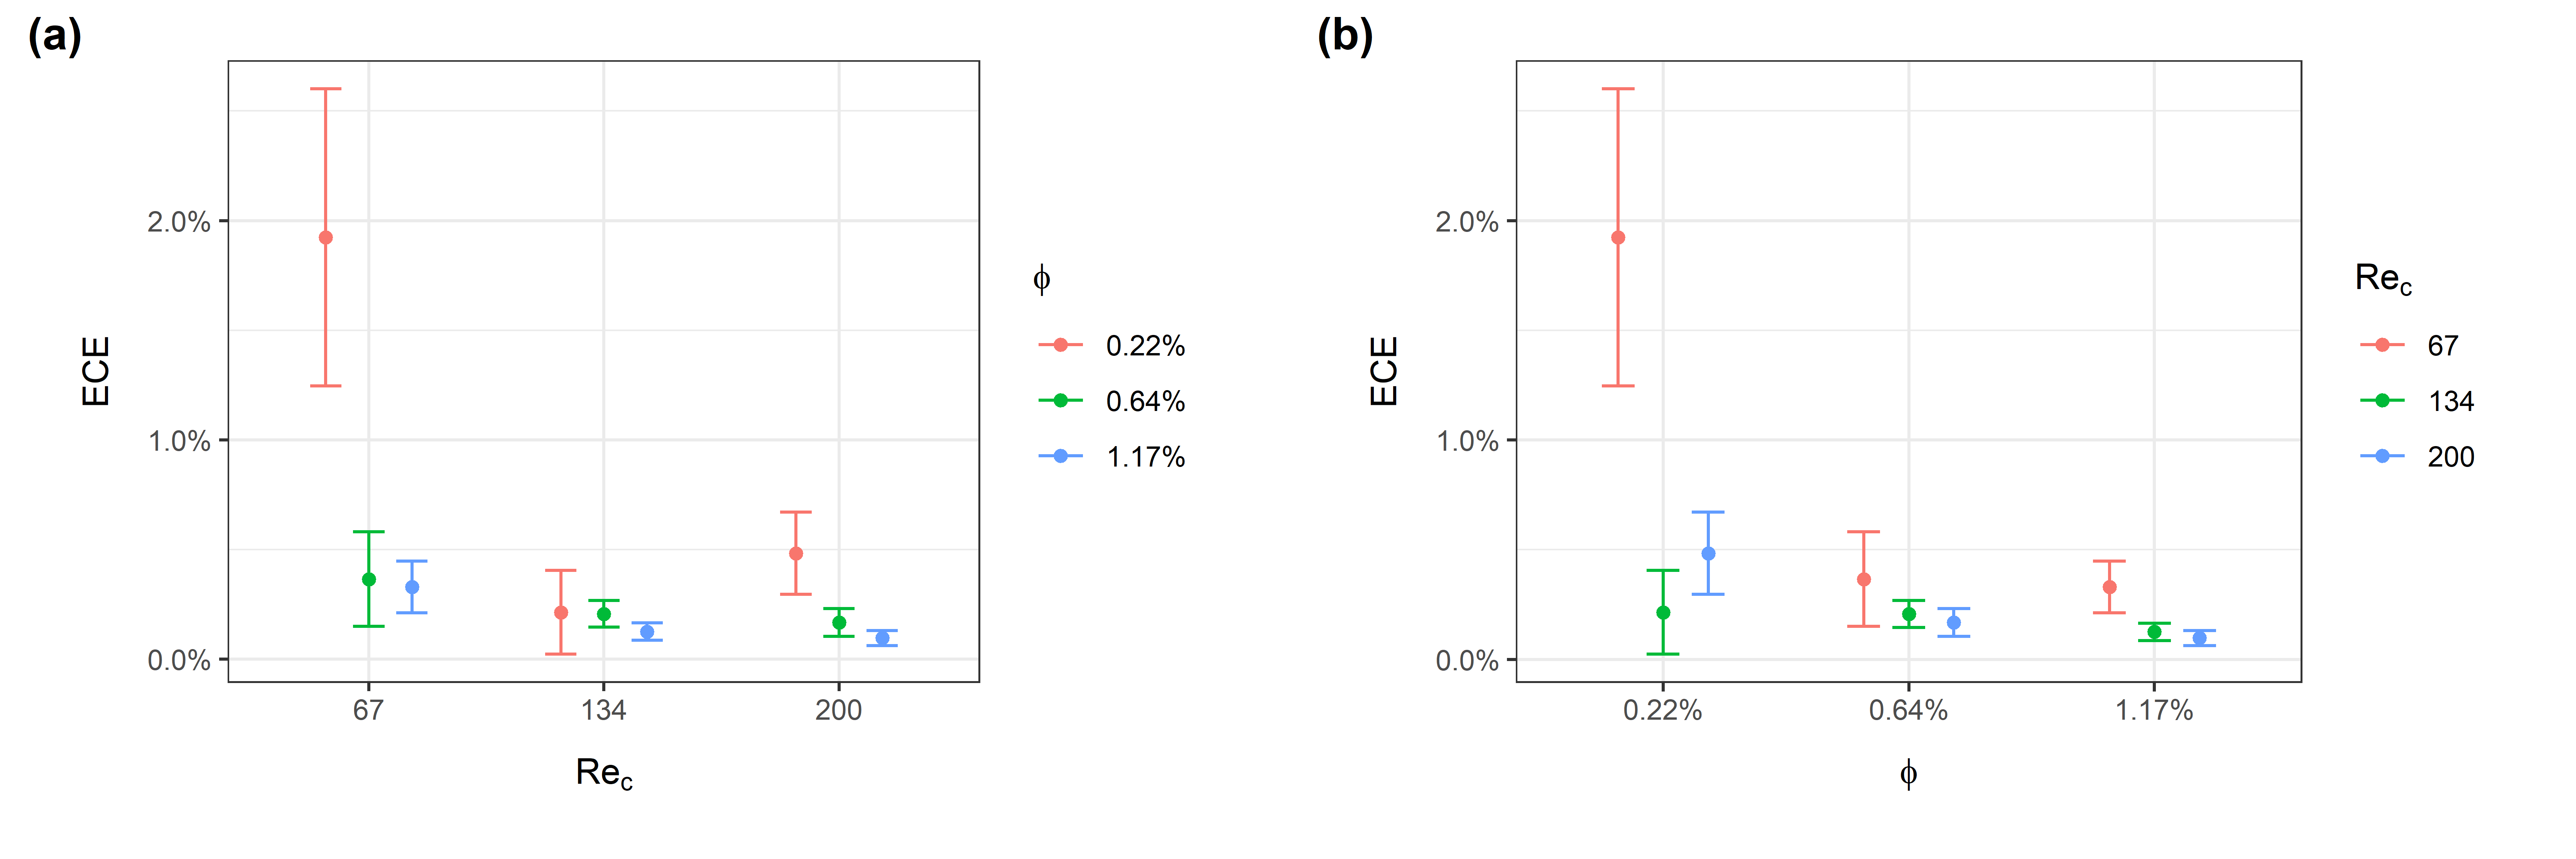
\includegraphics[width=5in]{../pics/ece_plot.png}
\caption{Estimates of effective capture efficiency calculated from laboratory experiments across the collector density $\times$ Reynolds number parameter space. Error bars represent +/- 1 SE. (\textbf{a}) Estimates plotted over $\Rey_c$, colored by solid volume fraction ($\phi_c$). (\textbf{b}) Estimates plotted over solid volume fraction, colored by $\Rey_c$.}
\label{fig:ece}
\end{figure}   

Monte Carlo analysis determined that there is a significant negative relationship between ECE and collector density for the low (p = 0.004) and high (p = 0.019) $\Rey_c$ treatments, but no significant effect was detected (p > 0.05) for the intermediate treatment (Figure \ref{fig:monte}a). We also found a significant negative relationship between ECE and $\Rey_c$ for the low (p = 0.026) and high (p = 0.046) collector-density treatments, but an insignificant (p > 0.05) trend for the intermediate collector-density treatment (Figure \ref{fig:monte}b). 

% Monte Carlo figure
\begin{figure}[H]
\centering
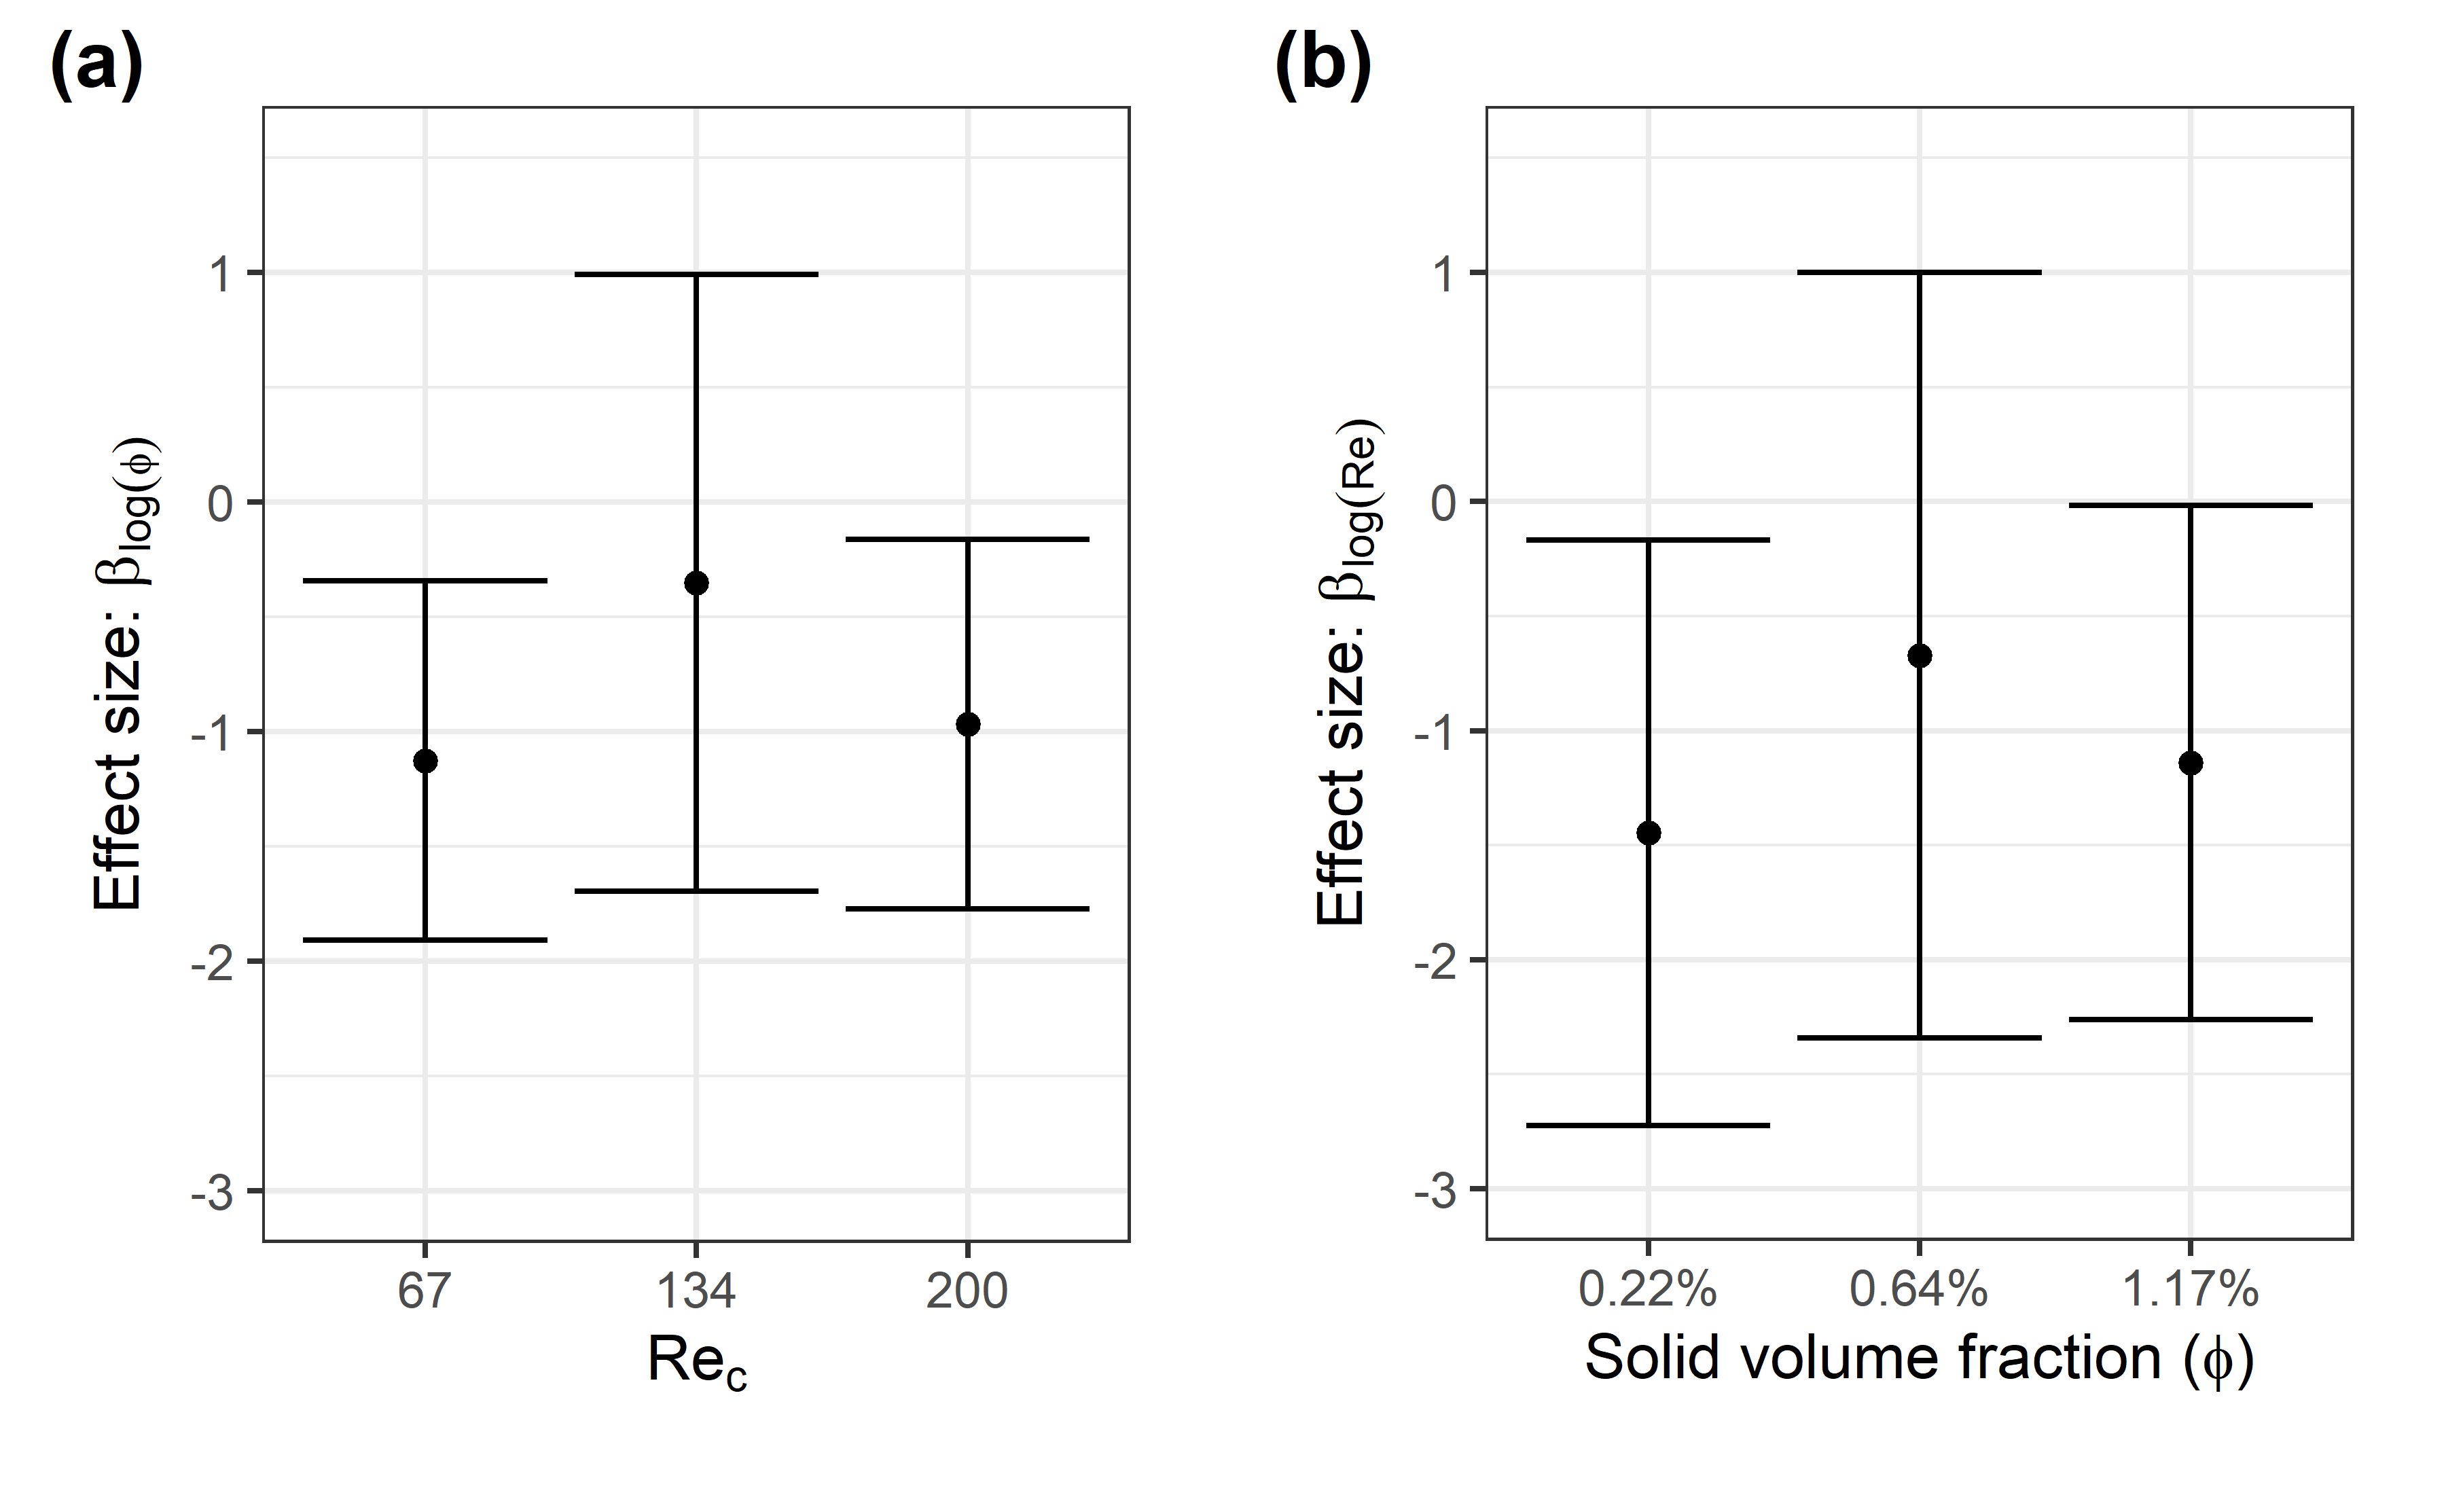
\includegraphics[width=5in]{../pics/montecarlo.png}
\caption{Effect size estimates from Monte Carlo regression analysis. Error bars represent 95\% confidence intervals. Asterisks mark the parameter values at which the effect size was found to be significant. (\textbf{a}) Estimates of the effect of log-transformed collector solid volume fraction ($\beta_{\log(\phi_c)}$) on ECE, stratified by $\Rey_c$. (\textbf{b}) Estimates of the effect of log-transformed $\Rey_c$ ($\beta_{\log(\Rey_c)}$) on ECE, stratified by solid volume fraction ($\phi_c$).}
\label{fig:monte}
\end{figure}   

\subsection{Turbulence and Flow Characteristics}

Turbulent kinetic energy was consistently found to increase with increasing flow velocity as expected (Table \ref{tbl:turbulence}). Generally, higher collector density also led to greater turbulence, with the greatest increase in terms of both absolute and relative magnitude taking place between the lower and middle collector-density treatments. A slight decrease actually occurred thereafter (between the middle and highest collector densities) for the middle and highest $\Rey_c$ treatments, with a slight increase for the lowest $\Rey_c$ treatment. Altogether, these results likely indicate that the turbulent eddy scale and the distance between collectors converged somewhere in our range for those parameters, so that additional collectors acted to damp eddies more than they acted to create them. If there is a threshold for this effect, our results, including the relative similarity between the lowest collector density and the zero-collector control, suggest that it would occur at a collector-density value between our lower and middle treatments.

% Turbulence table
\begin{table}[H]
\caption{Turbulent kinetic energy (TKE) for all collector solid volume fraction ($\phi_c$) and $\Rey_c$ treatments, including the control (zero-collector) treatments for reference.}
\centering
%% \tablesize{} %% You can specify the fontsize here, e.g., \tablesize{\footnotesize}. If commented out \small will be used.
\begin{tabular}{>{\bfseries}r>{\bfseries}rrr}
\toprule
\textbf{$\phi_c$}&\textbf{$\Rey_c$}&\textbf{mid-water-column TKE (\SI{}{\milli\metre^2/\second^2})}\\
\midrule
Control &   67  & \num{2.48}\\
        &   134 & \num{2.98}\\
        &   200 & \num{3.37}\\
\midrule
0.22\% &   67  & \num{1.23}\\
        &   134 & \num{5.26}\\
        &   200 & \num{12.2}\\
\midrule
0.64\% &   67  & \num{9.13}\\
        &   134 & \num{35.9}\\
        &   200 & \num{59.6}\\
\midrule
1.17\%  &   67  & \num{11.1}\\
        &   134 & \num{29.8}\\
        &   200 & \num{54.4}\\
\bottomrule
\label{tbl:turbulence}
\end{tabular}
\end{table}

\subsection{Biofilm Effects}

Biofilm growth was consistently found to increase ECE (Figure \ref{fig:biofilm}). The absolute increase was greatest by a considerable margin at the lowest collector density, for which biofilm was also allowed to grow for the shortest time. The middle and highest collector densities had similar absolute quantities of increase in their ECE for the initial biofilm runs (18-20 days), although the highest collector-density treatment demonstrated a far greater magnitude of increase in ECE after being allowed to grow for an additional 26 days (46 total).

% Biofilm figure
\begin{figure}[H]
\centering
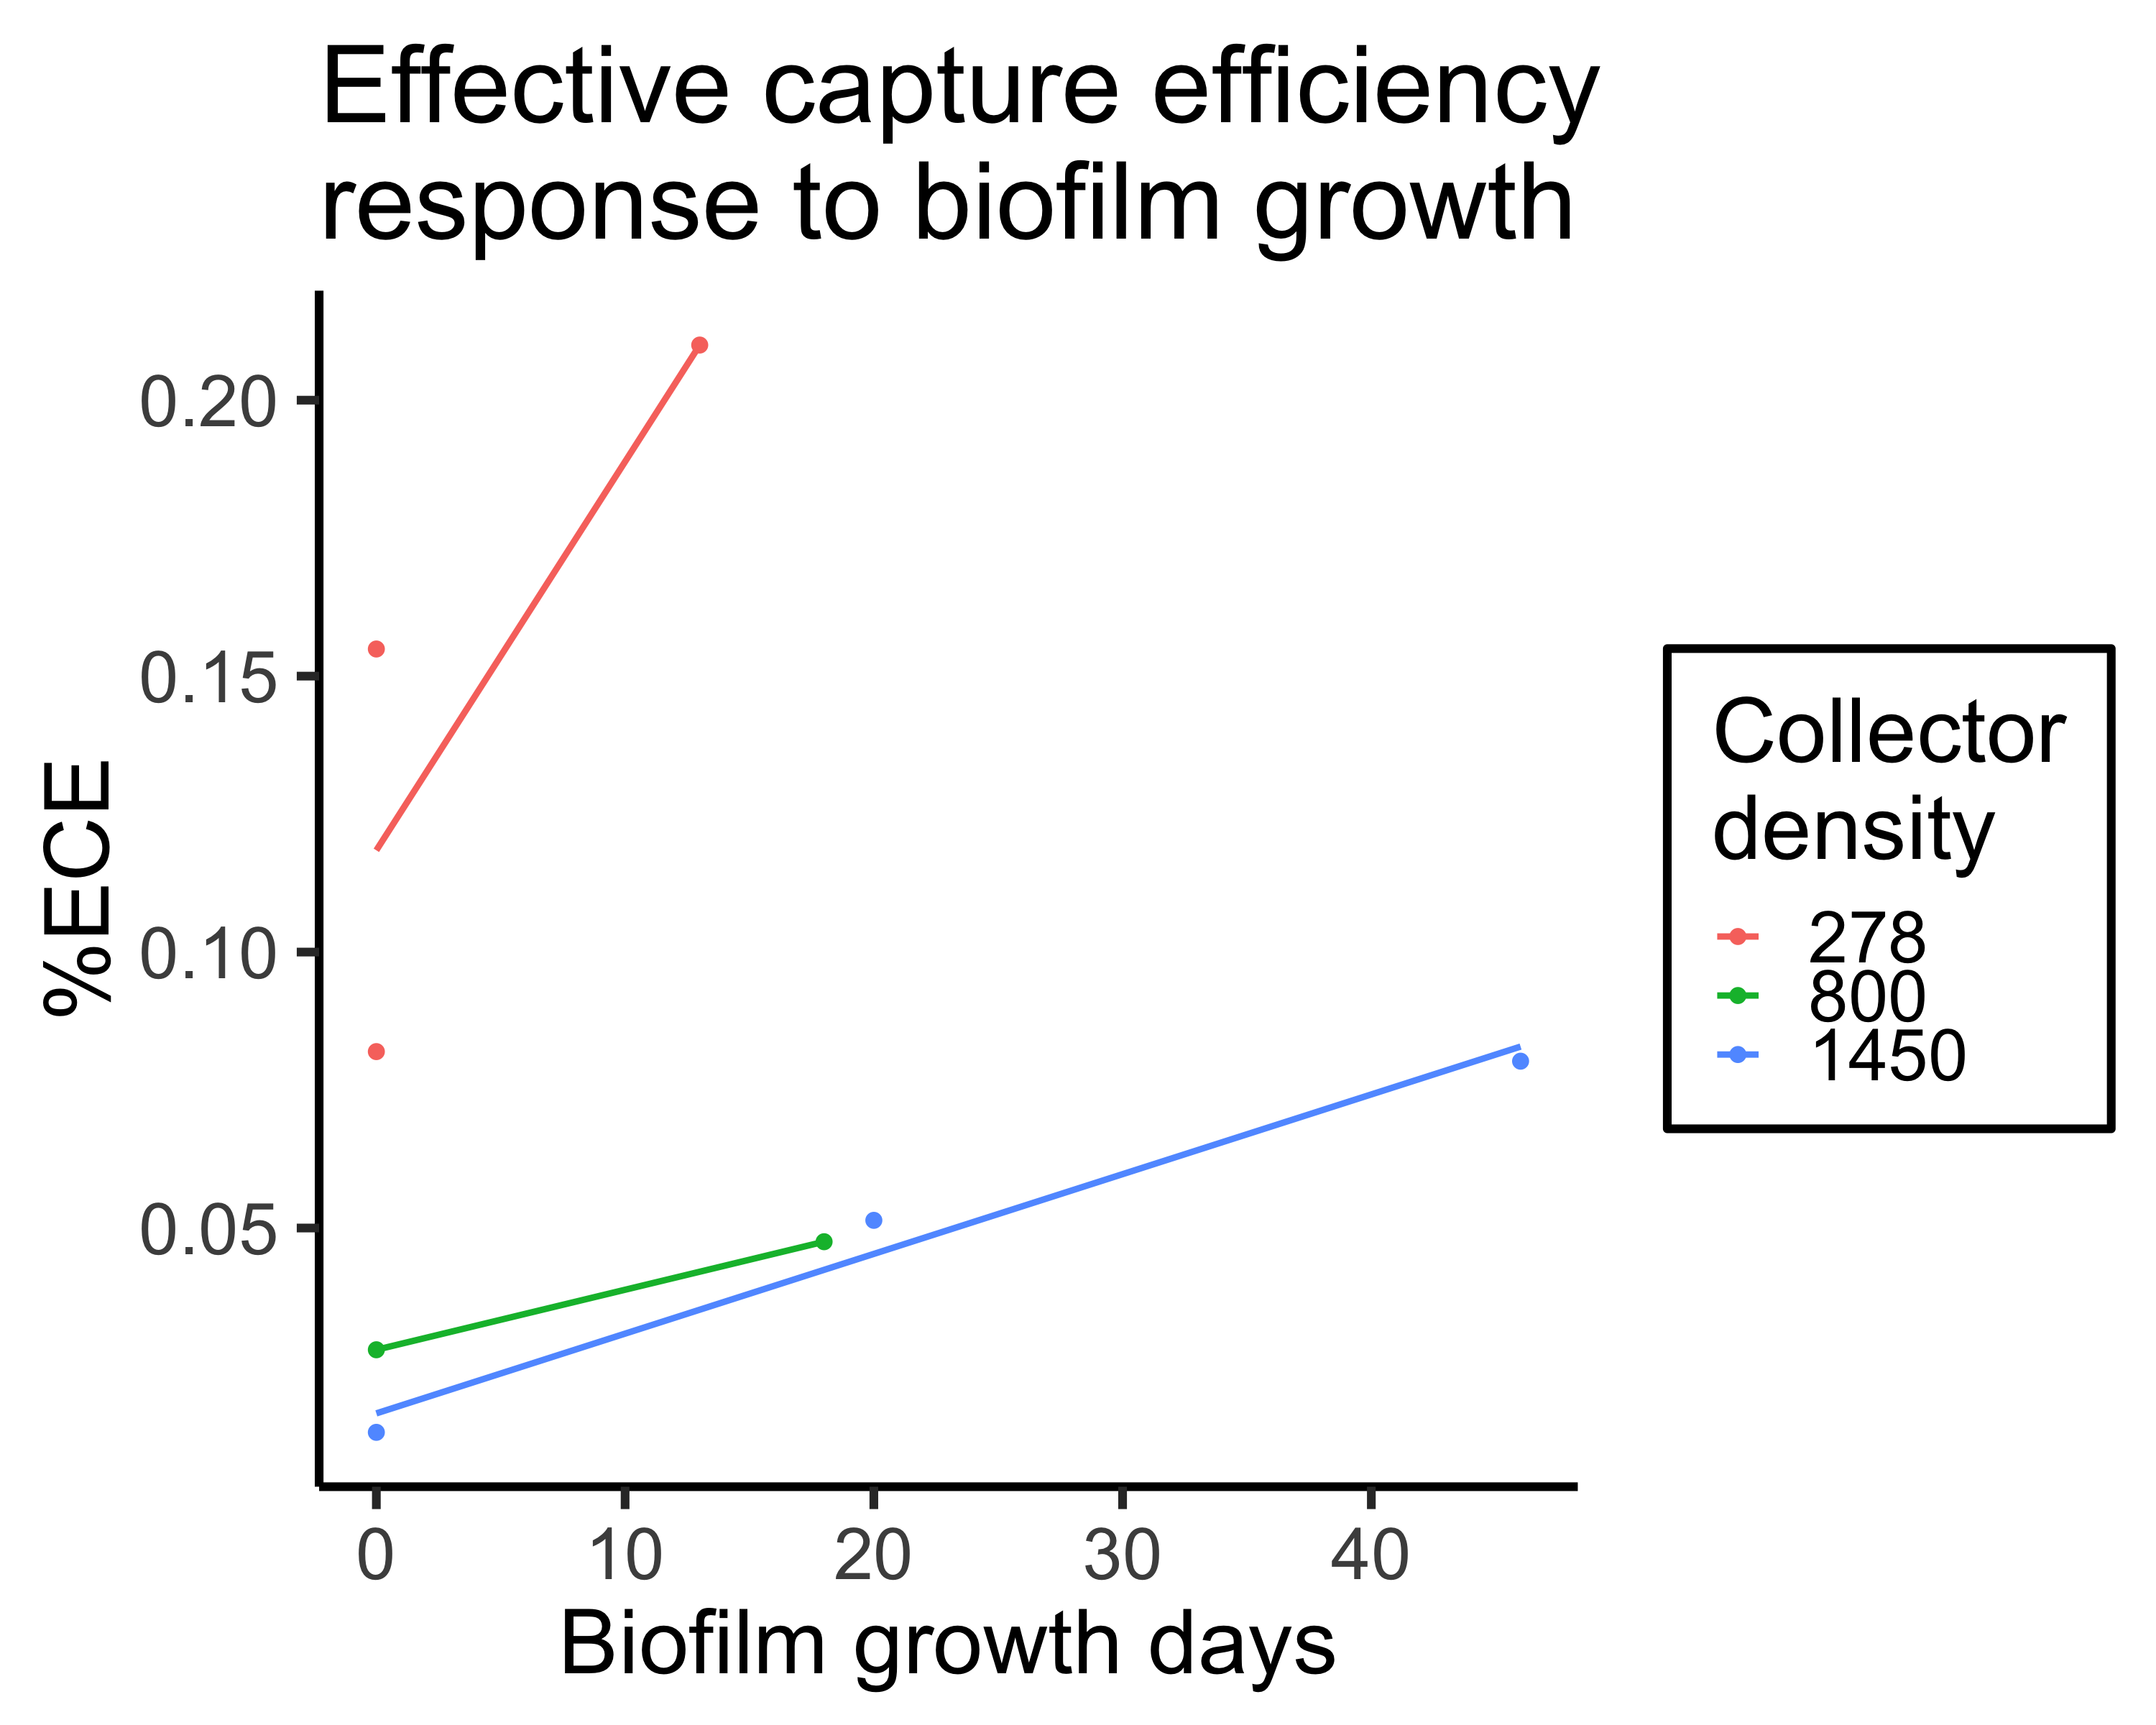
\includegraphics[width=5in]{../pics/biofilm.png}
\caption{Estimates of effective capture efficiency calculated from experimental runs with varying degrees of biofilm growth. Colors represent the different collector densities, expressed as solid volume fraction ($\phi_c$). Straight lines are drawn between the points that represent our experiments and the shaded areas represent 95\% confidence intervals for ECE inferred from our measurement uncertainty.}
\label{fig:biofilm}
\end{figure}   

\subsection{Comparison to Previous Models of Capture Efficiency}

Aside from the outlier at the mid $\Rey_c$, lowest collector-density treatment, all of our observations were in agreement with the power-law model adapted by Fauria et al. \cite{Fauria_2015} from Palmer \cite{Palmer_2004} (Figure \ref{fig:compplot}). In no other case did the model prediction differ from our empirical observation by more than 1 standard error (SE), which is likely attributable to measurement error and/or stochastic variance implicit in our physical experiments.

% Fauria model comparison figure
\begin{figure}[H]
\centering
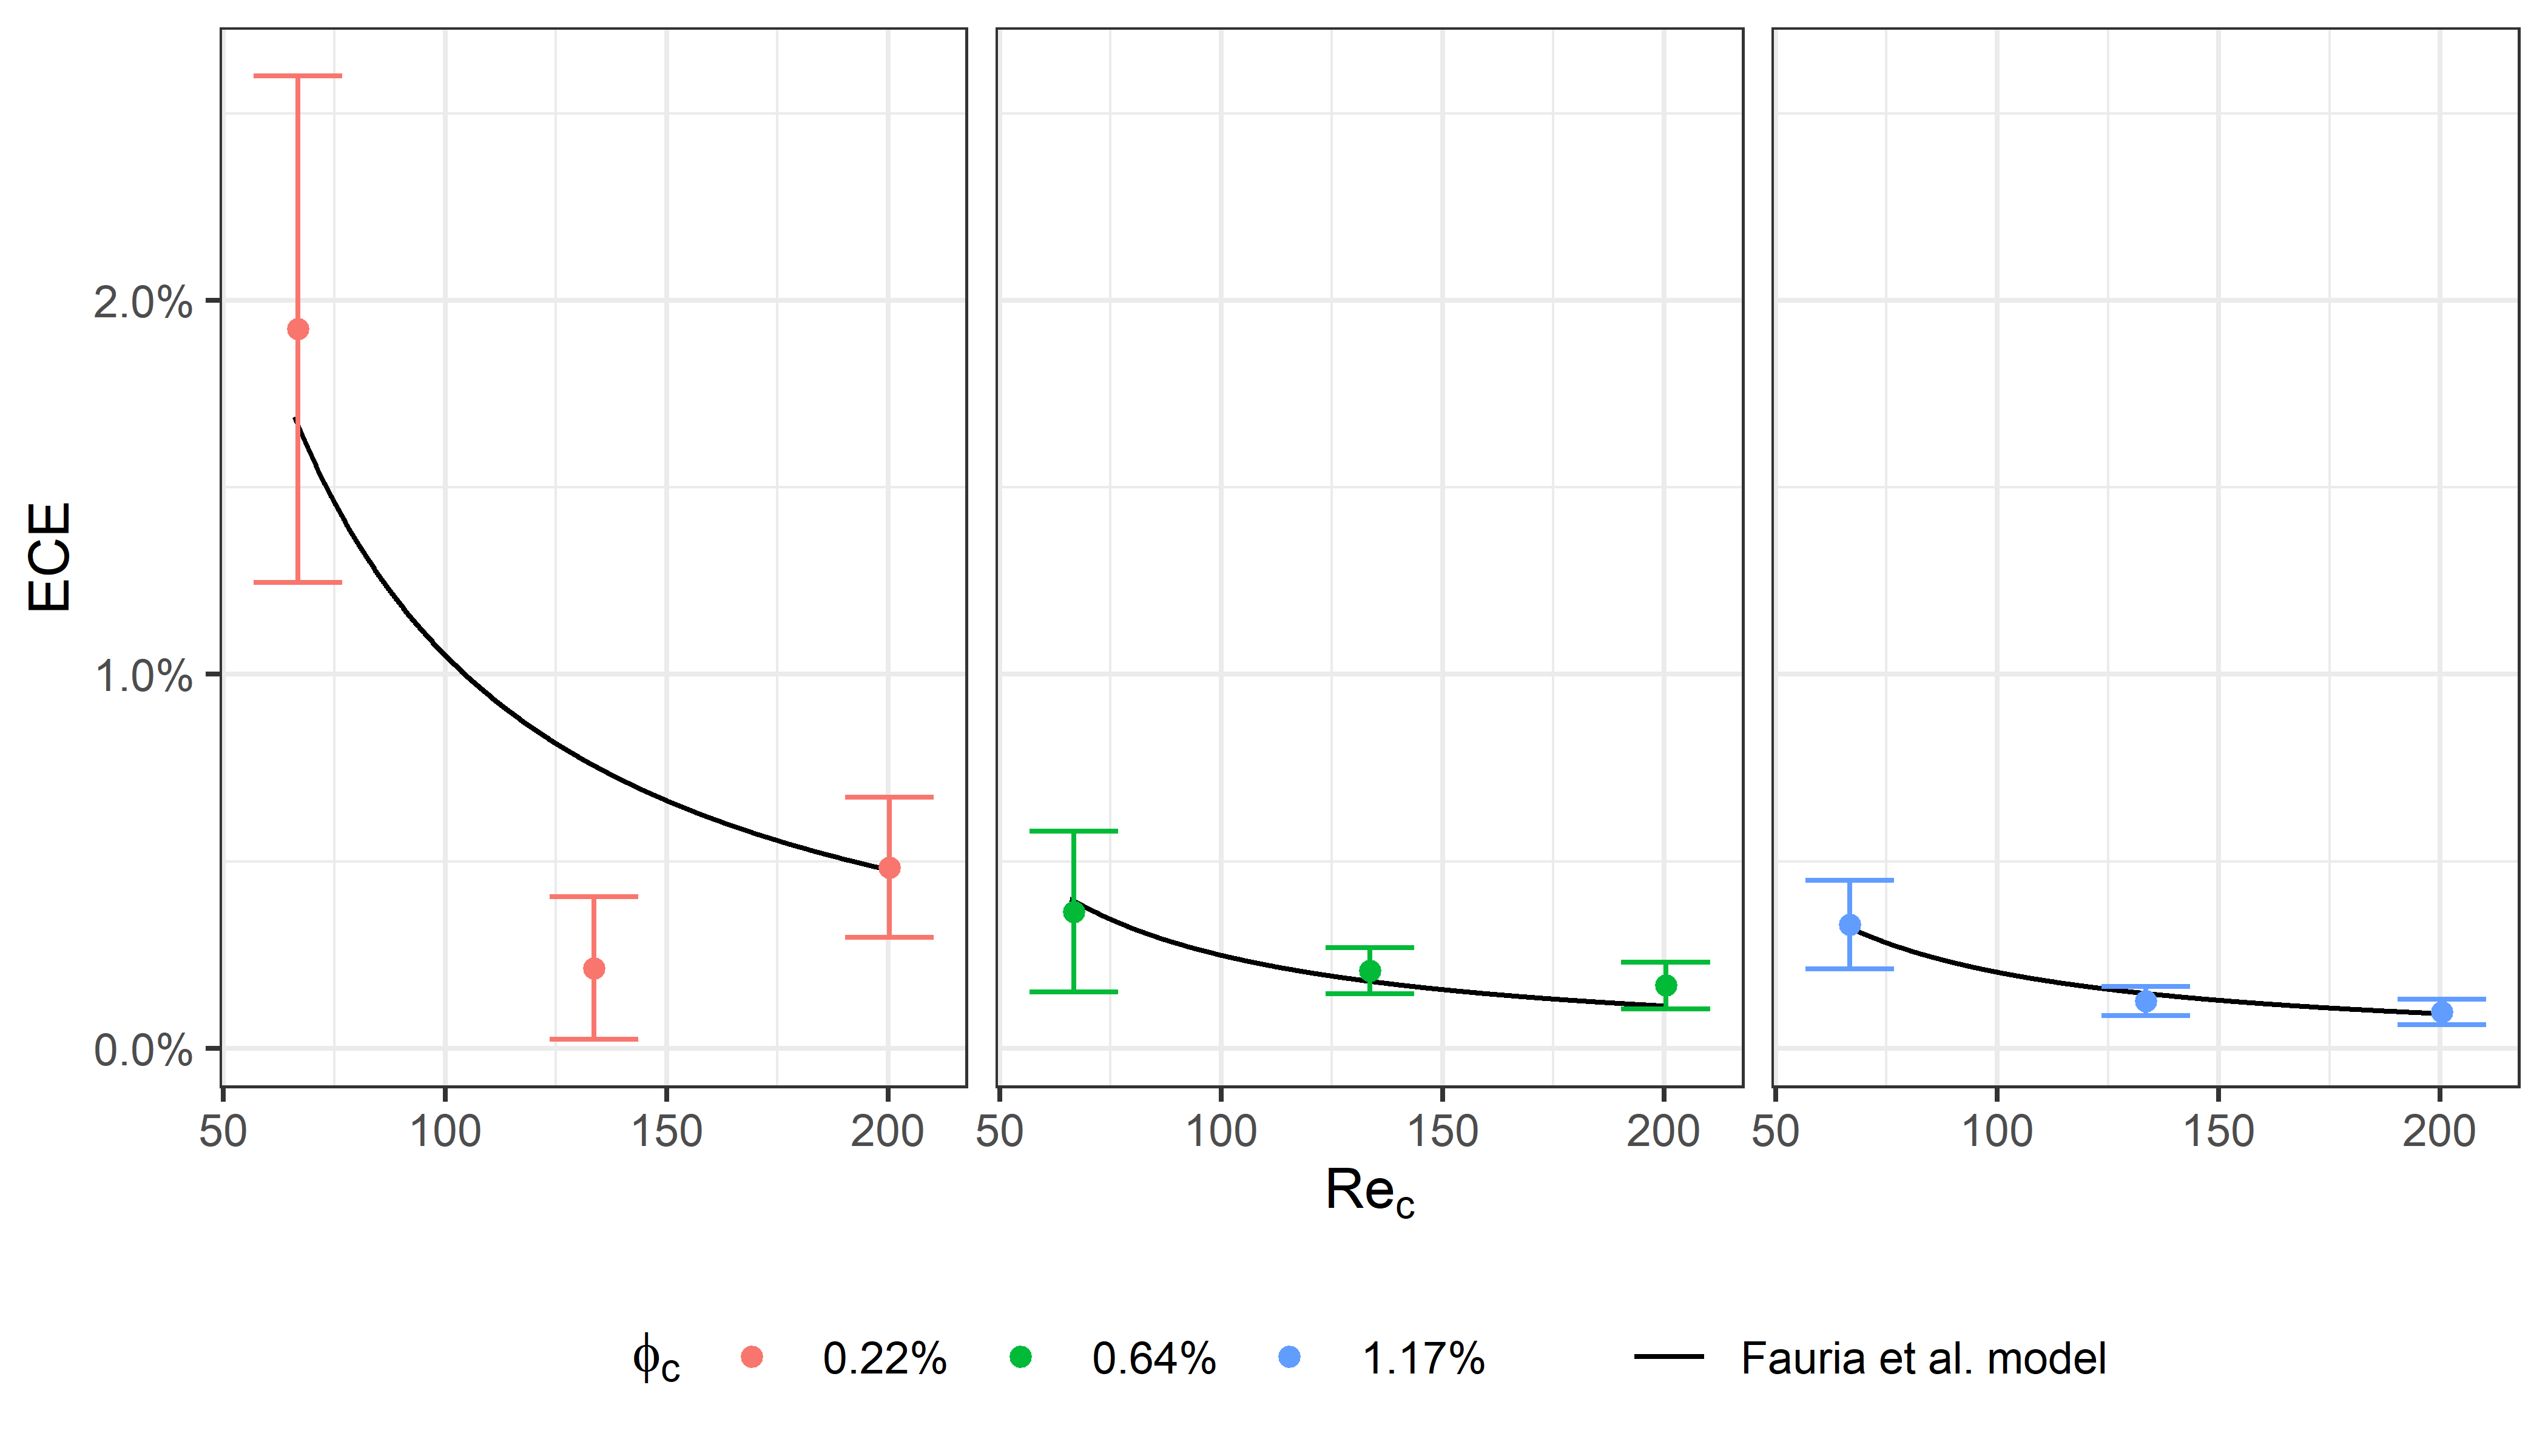
\includegraphics[width=5in]{../pics/comparisonplot.png}
\caption{A comparison of our experimental estimates of effective capture efficiency, colored according to collector solid volume fraction ($\phi_c$), and the predictions of the Fauria et al. \cite{Fauria_2015} power law model (black lines). Effective capture efficiency is plotted on a log scale in order to display model fit more accurately at small values. Error bars represent +/- 1 SE.}
\label{fig:compplot}
\end{figure}   

Having confirmed that the Fauria et al. \cite{Fauria_2015} model is a reasonably good predictor for our results, we found the $C$ values for our different collector-density treatments and compared them to those estimated for the two collector densities studied by Fauria et al. ($\phi_c$ = 0.82\%, 2.16\%). We then fit a preliminary power-law regression to the results at the two studies' five combined $\phi_c$ test values, which fit relatively well (R$^2$ = 0.82) though data scarcity and the differing environments of the two studies are important to consider in evaluating the certainty of this model's coefficients.

% C-phi model figure
\begin{figure}[H]
\centering
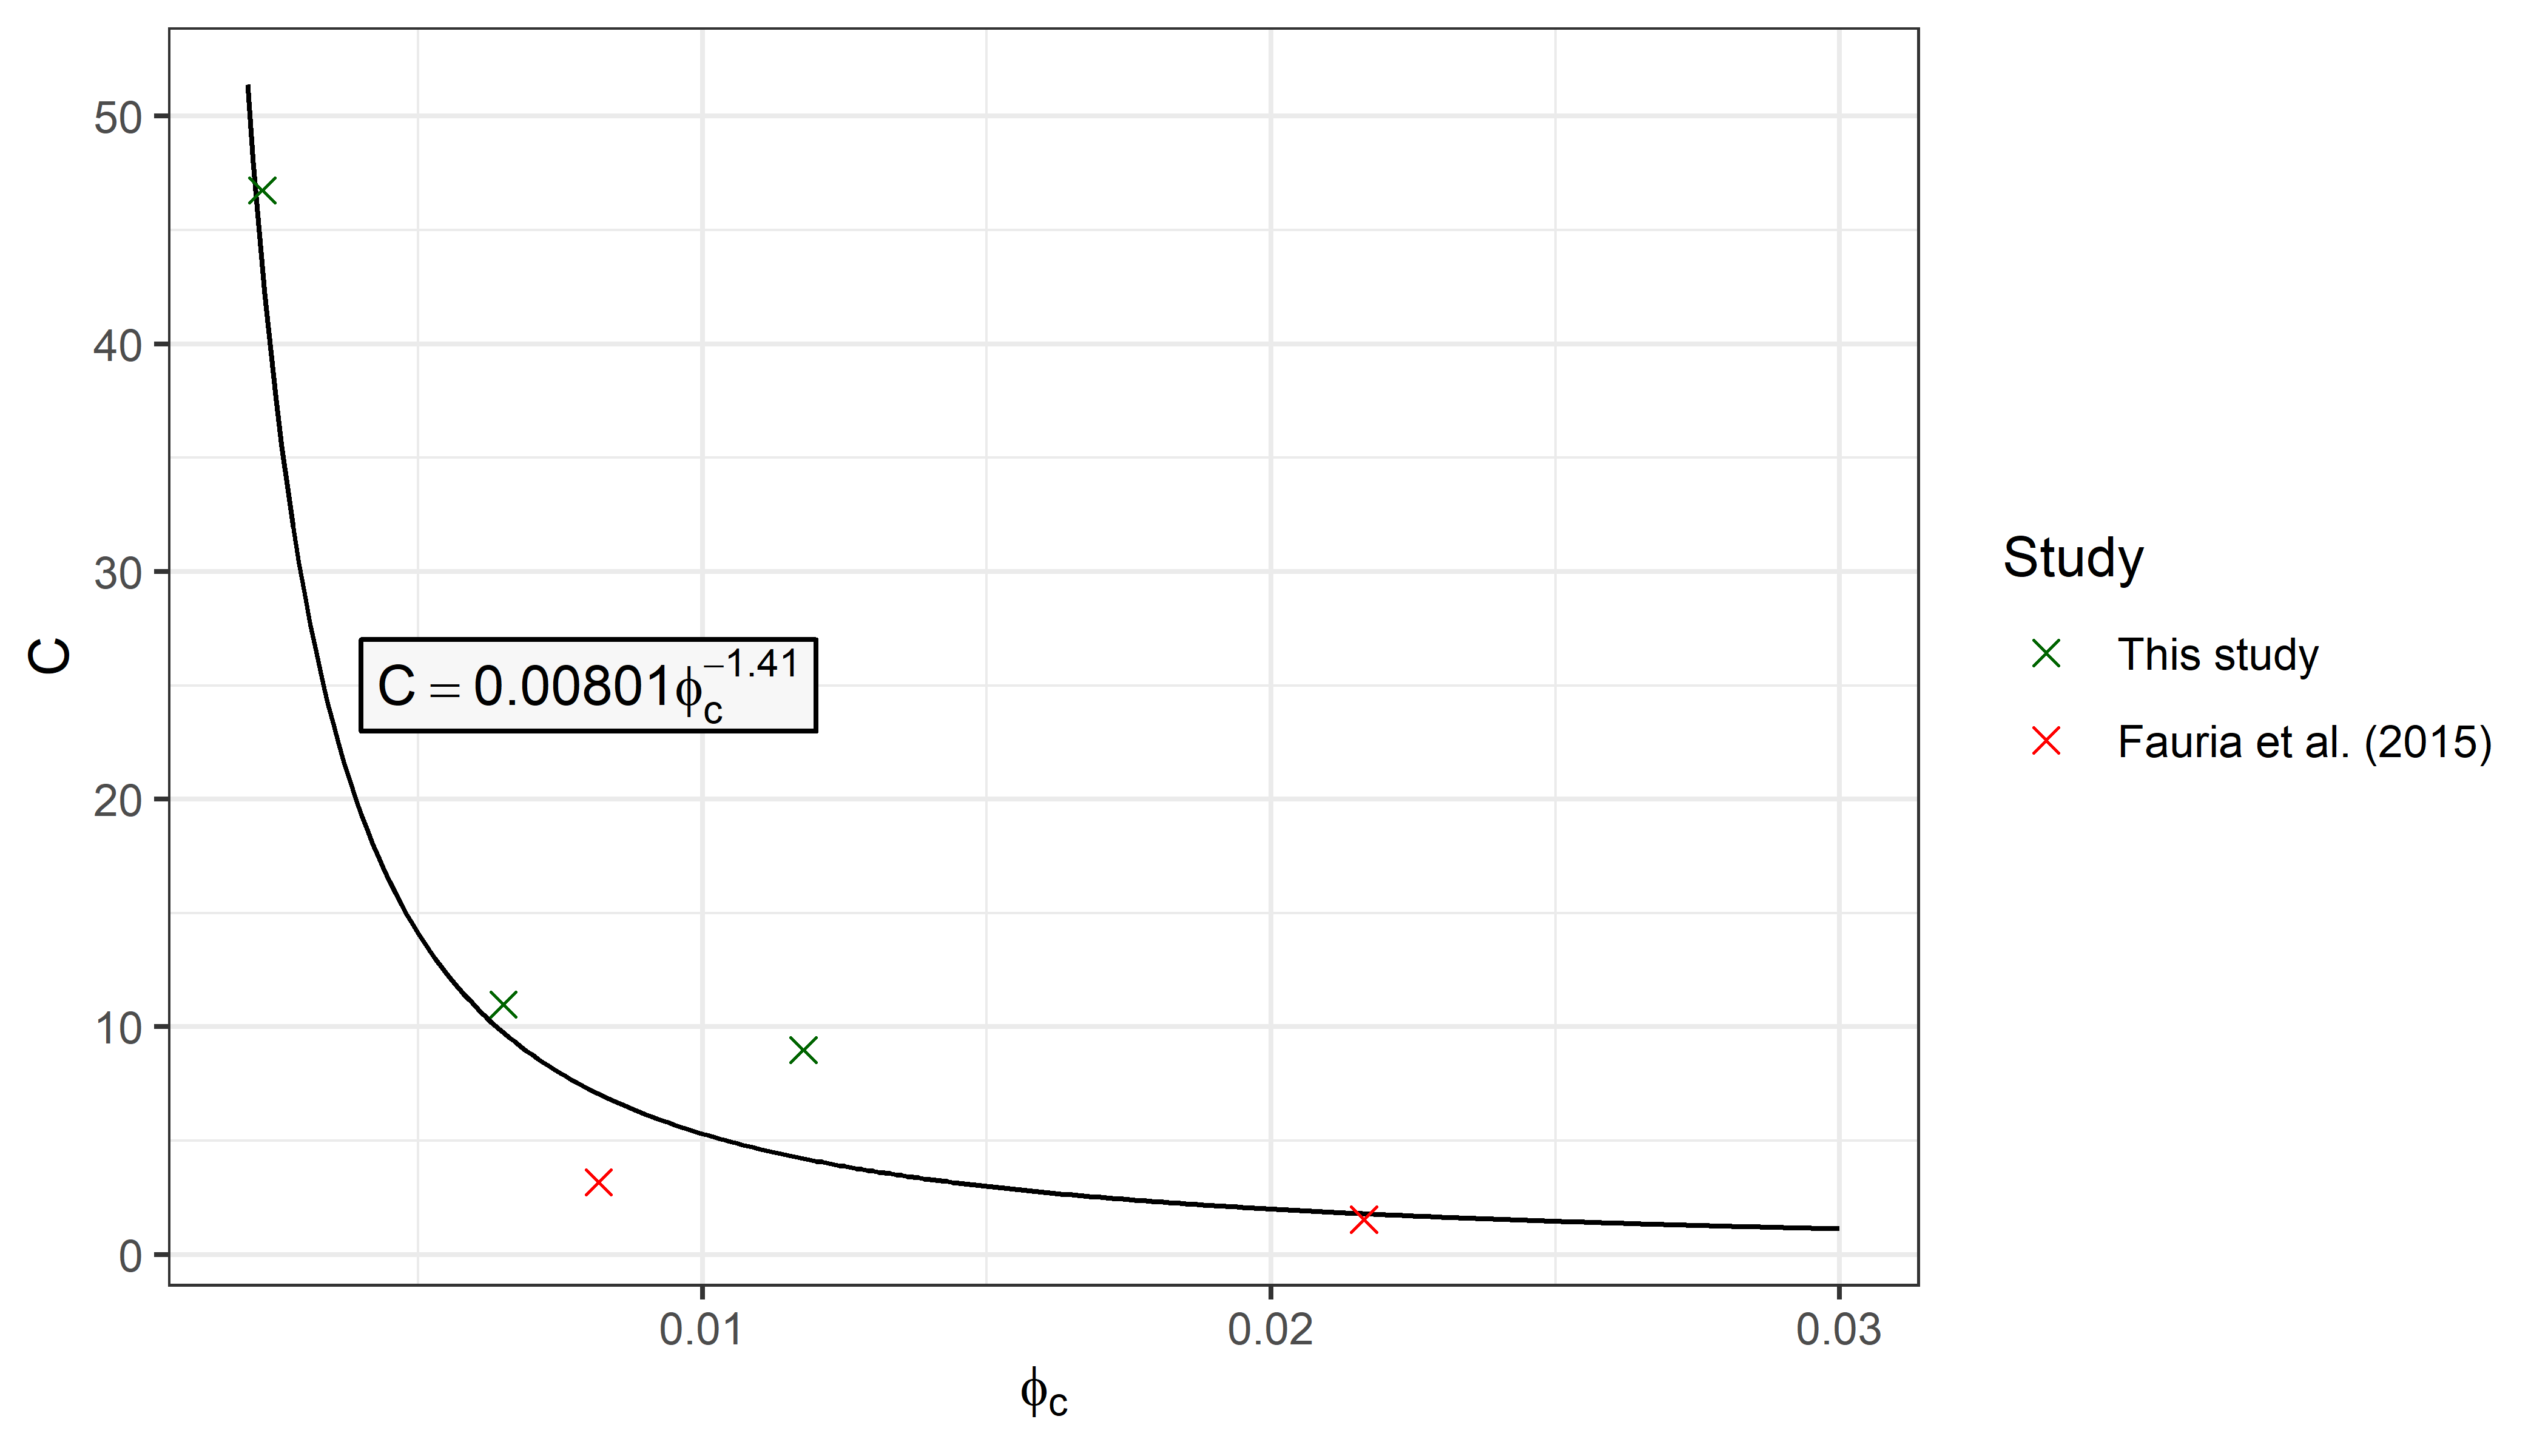
\includegraphics[width=5in]{../pics/cphiplot.png}
\caption{A comparison of the $C$ values calculuated for each of our collector-density treatments to those calculated by Fauria et al. \cite{Fauria_2015}. The black line represents the power law model of best fit between $C$ and collector solid volume fraction ($\phi_c$) for our collector-density treaments and those of Fauria et al. combined (n = 5), for which R$^2$ = 0.82.}
\label{fig:cphi}
\end{figure}   

\section{Discussion}

\subsection{Inferred Mechanisms of Effect for Collector Density and Reynolds Number}

\subsection{Relative Importance of Biofilm}

\subsection{Designing Wetlands for Maximum Sedimentation}

\vspace{6pt} 

%%%%%%%%%%%%%%%%%%%%%%%%%%%%%%%%%%%%%%%%%%
%% optional
\supplementary{The following are available online at \linksupplementary{s1}, Figure S1: title, Table S1: title, Video S1: title.}

% Only for the journal Methods and Protocols:
% If you wish to submit a video article, please do so with any other supplementary material.
% \supplementary{The following are available at \linksupplementary{s1}, Figure S1: title, Table S1: title, Video S1: title. A supporting video article is available at doi: link.}

\authorcontributions{Conceptualization, L.L., J.N., and J.W.; methodology, L.L. and J.W.; software, L.L., J.N., J.W., and C.Y.; validation, J.W.; formal analysis, J.W. and C.Y.; investigation, J.N., J.W, and C.Y.; resources, L.L.; data curation, J.W.; writing--original draft preparation, J.N., J.W., and C.Y.; writing--review and editing, L.L., J.N., J.W., and C.Y.; visualization, J.W.; supervision, L.L., J.W., and C.Y.; project administration, L.L. and J.W.; funding acquisition, L.L.}

\funding{This research was funded by NSF award \#1455362.}

\acknowledgments{The authors wish to thank and acknowledge Colin Keating and Aaron Hurst for their helpful work on preliminary flume experiments. We also wish to express great thanks to Yayla Sezinger, Elle Chen, Nicole Ulakovic, Katrina Ginsberg, and Danielle Satin for their time spent preparing for experiments, maintaining the flume, and fastidiously carrying out other important laboratory tasks. Lastly, we wish to thank Sam Stein and Sheila Trampush for graciously sharing data and participating in brainstorming sessions while working on concurrent studies within the same general topic area.}

\conflictsofinterest{The authors declare no conflict of interest.} 

%% optional
% \abbreviations{The following abbreviations are used in this manuscript:\\

% \noindent 
% \begin{tabular}{@{}ll}
% MDPI & Multidisciplinary Digital Publishing Institute\\
% DOAJ & Directory of open access journals\\
% TLA & Three letter acronym\\
% LD & linear dichroism
% \end{tabular}}

%%%%%%%%%%%%%%%%%%%%%%%%%%%%%%%%%%%%%%%%%%
%% optional
% \appendixtitles{no} %Leave argument "no" if all appendix headings stay EMPTY (then no dot is printed after "Appendix A"). If the appendix sections contain a heading then change the argument to "yes".
% \appendix
% \section{}
% \unskip
% \subsection{}
% The appendix is an optional section that can contain details and data supplemental to the main text. For example, explanations of experimental details that would disrupt the flow of the main text, but nonetheless remain crucial to understanding and reproducing the research shown; figures of replicates for experiments of which representative data is shown in the main text can be added here if brief, or as Supplementary data. Mathematical proofs of results not central to the paper can be added as an appendix.

% \section{}
% All appendix sections must be cited in the main text. In the appendixes, Figures, Tables, etc. should be labeled starting with `A', e.g., Figure A1, Figure A2, etc. 

%%%%%%%%%%%%%%%%%%%%%%%%%%%%%%%%%%%%%%%%%%
% Citations and References in Supplementary files are permitted provided that they also appear in the reference list here. 

%=====================================
% The following MDPI journals use author-date citation: Arts, Econometrics, Economies, Genealogy, Humanities, IJFS, JRFM, Laws, Religions, Risks, Social Sciences. For those journals, please follow the formatting guidelines on http://www.mdpi.com/authors/references
% To cite two works by the same author: \citeauthor{ref-journal-1a} (\citeyear{ref-journal-1a}, \citeyear{ref-journal-1b}). This produces: Whittaker (1967, 1975)
% To cite two works by the same author with specific pages: \citeauthor{ref-journal-3a} (\citeyear{ref-journal-3a}, p. 328; \citeyear{ref-journal-3b}, p.475). This produces: Wong (1999, p. 328; 2000, p. 475)

% =====================================
% References, variant B: external bibliography
% =====================================

\reftitle{References}
\externalbibliography{yes}
\bibliography{refs}

%%%%%%%%%%%%%%%%%%%%%%%%%%%%%%%%%%%%%%%%%%
%% optional
%\sampleavailability{Samples of the compounds ...... are available from the authors.}

%% for journal Sci
%\reviewreports{\\
%Reviewer 1 comments and authors’ response\\
%Reviewer 2 comments and authors’ response\\
%Reviewer 3 comments and authors’ response
%}

%%%%%%%%%%%%%%%%%%%%%%%%%%%%%%%%%%%%%%%%%%

\end{document}
